%
% CMPT 379: Principles of Compiler Design - A Course Overview
%
% Author: Jeffrey Leung
%

\documentclass[10pt, oneside, letterpaper, titlepage]{article}

\usepackage{amsmath}
\usepackage[ampersand]{easylist}
	\ListProperties(
		Progressive*=5ex,
		Space=5pt,
		Space*=5pt,
		Style1*=\textbullet\ \ ,
		Style2*=\begin{normalfont}\begin{bfseries}\textendash\end{bfseries}\end{normalfont} \ \ ,
		Style3*=\textasteriskcentered\ \ ,
		Style4*=\begin{normalfont}\begin{bfseries}\textperiodcentered\end{bfseries}\end{normalfont}\ \ ,
		Style5*=\textbullet\ \ ,
		Style6*=\begin{normalfont}\begin{bfseries}\textendash\end{bfseries}\end{normalfont}\ \ ,
		Style7*=\textasteriskcentered\ \ ,
		Style8*=\begin{normalfont}\begin{bfseries}\textperiodcentered\end{bfseries}\end{normalfont}\ \ ,
		Hide1=1,
		Hide2=2,
		Hide3=3,
		Hide4=4,
		Hide5=5,
		Hide6=6,
		Hide7=7,
		Hide8=8 )
\usepackage[T1]{fontenc}
\usepackage{forest}
\usepackage{geometry}
	\geometry{margin=1.2in}
\usepackage{graphicx}
	\graphicspath{ {img/} }
\usepackage[colorlinks=true, linkcolor=blue]{hyperref}
\usepackage{listings}
\usepackage{lmodern} % Allows the use of symbols in font size 10; http://ctan.org/pkg/lm
\usepackage{multirow}
\usepackage{textcomp} % Allows the use of \textbullet with the font
\usepackage{verbatim}

\renewcommand{\arraystretch}{1.2}
\renewcommand{\familydefault}{\sfdefault}

\title{CMPT 379: Principles of Compiler Design \\\medskip \Large A Course Overview}
\author{Jeffrey Leung \\ Simon Fraser University}
\date{Summer 2019}

\begin{document}

	\maketitle
	\tableofcontents
	\clearpage

	%
% CMPT 213: Object Oriented Design in Java - A Course Overview
% Section: Introduction
%
% Author: Jeffrey Leung
%

\section{Introduction}
	\label{sec:introduction}
\begin{easylist}

& Standards:
	&& Make fields private when possible

& Commenting:
	&& Comment purpose of a class
	&& Name fields/methods/parameters so comments are unnecessary

& When possible, convert strings to non-string types internally for consistency

& \textbf{Clean code:} Code which is correct, easy to read/maintain, and conforms to a standard

& Software design:
	&& 4 steps:
		&&& Requirements
		&&& Design and implementation
		&&& Verification
		&&& Evolution
	&& Designing involves identifying classes, responsibilities, and relationships to create a diagram
	&& Implementation process options:
		&&& \textbf{Skeleton code:} Beginning minimal parts/features of a system
		&&& \textbf{Component-wise:} Creating components one at a time
	&& Methods of integrating code from multiple people:
		&&& \textbf{Continual integration:} Gradual system growth by constantly integrating changes
		&&& \textbf{Big Bang integration:} Building all parts separately without integrating until the end

& \textbf{Feature envy:} Characteristic of a class which relies heavily on another class
& Warning sign: Characteristic of a method which operates more strongly on another object than its own
& \textbf{Deprecation:} State where a public interface is no longer supported or recommended, and is slated to be removed in the future


& \textbf{try-catch:} Structure which watches for an exception and handles it
	&& Only one exception can be live at a given time
	&& \textbf{finally clause:} Optional clause after catch clauses which is executed regardless of the result
		&&& If exception is thrown, the finally clause is executed immediately afterwards
	&& \textbf{try-with-resources:} Block which cleans up a resource when a try block exits

& Exception: Issue which may be fixable and is not out of the software's control
	&& \textbf{Checked exception:} Exception which must be caught or listed in a throws clause
	&& \textbf{Unchecked exception:} Exception which will automatically propagate and does not require catching
		&&& E.g. RuntimeException
		&&& Preferred as it does not require modification of methods between try/catch, which decouples code

\end{easylist}
\clearpage

	%
% CMPT 379: Principles of Compiler Design - A Course Overview
% Section: Lexical Analysis (Scanning)
%
% Author: Jeffrey Leung
%

\section{Lexical Analysis (Scanning)}
	\label{sec:lexical-analysis}
\begin{easylist}

& \textbf{Lexical analysis (scanning):} Transforming an input program string into tokens
	&& Does not validate, simply transforms
	&& Challenges:
		&&& Prove that the implementation captures all tokens specified by the language definition
		&&& Prove correctness of transformations

& \textbf{Token:} Symbol which represents a specific composable section of code
	&& E.g. Open bracket, number
	&& Can be denoted as \lstinline{T_IDENT}, \lstinline{T_LPAREN}, etc.
	&& \textbf{Lexeme/token attribute:} Value of a token
		&&& Not all tokens have values
		&&& E.g. For \lstinline{T_INTCONSTANT}, a possible value is 1
	&& The same character should only represent a single token (e.g. \lstinline{-} should be represented by the same token whether it is a unary or binary operator)

& \textbf{Loop and switch scanner:} Lexical analyzer which loops over each character sequentially and categorizes it based on context

\end{easylist}
\subsection{Regular Expressions}
	\label{subsec:reg-ex}
\begin{easylist}

& \textbf{Formal language:} A valid set of strings from a given alphabet of symbols
	&& \textbf{Symbol:} Single distinct character
		&&& \textbf{Alphabet:} The finite set of symbols
			&&&& Denoted by $\sum$ or $\{\textrm{symbol}\}$
	&& \textbf{String:} Sequence of symbols
		&&& \textbf{Empty string:} $\varepsilon$
		&&& Set of all strings: $\sum *$

& \textbf{Formal grammar:} Concise description of a formal language

& \textbf{Regular language:} A formal language which can be expressed through specific operations (i.e. any regular expression)
	&& For each regular language, there is an equivalent finite-state automaton
	&& The set of all regular languages includes:
		&&& The empty set
		&&& $\{a\}$ for all $a$ in $\sum \varepsilon$
		&&& For $L_1, L_2, L$ which are regular languages:
			&&&& Concatenation of $L_1 \cdot L_2$ where $\{xy | x \in L_1 \textrm{ and } y \in L_2\}$
			&&&& Union of $L_1 \cup L_2$
			&&&& Kleene closure as $L^* = \bigcup_{i=0}^{\infty} L^i$
		&&& No other regular languages

& \textbf{Regular expression:} Concise description of a regular language
	&& E.g. The set of all strings over the alphabet $\{a, b\}$ which end in $abb$ is expressed by $(a|b)*abb$
	&& Used to define tokens
	&& Core operators:
		&&& \textbf{Alternation:} One of several options
			&&&& E.g. $a|b = a \textrm{ or } b$ is a regular expression where $a, b$ are regular expressions
		&&& \textbf{Concatenation:} Combination of multiple regular expressions
			&&&& E.g. $ab$, a concatenation of $a$ and $b$, is a regular expression where $a, b$ are regular expressions
		&&& \textbf{Repetition:} An arbitrary amount of a regular expression
			&&&& E.g. $a*$, any number of $a$ regular expressions, is a regular expression
	&& Used in lexical analysis to match the largest valid string
	&& Can be expressed as a recursive tree structure or as a finite state automaton

\end{easylist}
\subsection{Finite State Automata}
\label{subsec:finite-state-automata}
\begin{easylist}

& \textbf{Finite State Automaton:} System consisting of a finite set of states and a transition function between states
	&& Notations:
		&&& Alphabet of symbols: $\Sigma$
		&&& Finite set of states: $S$
		&&& Start state: Outlined
		&&& Final/accepting state: Double-outlined
		&&& Transition function: $\sigma: S \times \Sigma = S$
	&& Equivalent to a unique regular language
  	&& Transition of $\epsilon$ refers to no input from the string corresponding to a transition in state
		&&&& Non-deterministic

& \textbf{Deterministic Finite Automata (DFA):} Finite State Automata where no state has more than one transition per input, and no $\epsilon$ moves exist
	&& For any given string, only one path exists from the start state to the final state
	&& Runtime complexity: $O(r^s)$
& \textbf{Nondeterministic Finite Automata (NFA):} Finite State Automata where at least one state has more than one transition per input, or an $\epsilon$ move exists
	&& For any given string, multiple paths may exist from the state state to the final state
	&& Usually larger than DFA
	&& Runtime complexity: $O(2^r)$ where $r$ is the initial cost of creating the automaton
	&& \textbf{Subset Construction:} Process to convert an NFA into a DFA
		&&& From the set of start states, given any input in the alphabet, output the set of potential resulting states. Repeat until no new sets of states are generated. Use each of the unique potential sets of states as a single DFA state.
		&&& Runtime complexity: Can convert regex of size $r$ to a $2^r$ state DFA

\end{easylist}
\clearpage

	%
% CMPT 379: Principles of Compiler Design - A Course Overview
% Section: Syntax Analysis (Parsing)
%
% Author: Jeffrey Leung
%

\section{Syntax Analysis (Parsing)}
	\label{sec:syntax-analysis}
\begin{easylist}

& \textbf{Syntax analysis (parsing):} Translation of a set of strings into a valid structure using a grammar
	&& \textbf{Language:} Description of a valid string of tokens

& Symbols and rules:
	&& \textbf{Terminal symbol:} Token or base symbol which does not represent any other symbols
	&& \textbf{Non-terminal symbol:} Set of strings potentially consisting of one or more terminal or non-terminal symbols
	&& \textbf{Production/Rule/Production rule:} Function on a non-terminal symbol which generates a sequence of terminal and/or non-terminal symbols
		&&& \textbf{Expansion:} Sequence of symbols resulting from the application of a production rule

\end{easylist}
\subsection{Context-Free Grammars}
	\label{subsec:syntax-analysis:context-free-grammars}
\begin{easylist}

& \textbf{Context-Free Grammar (CFG):} Recursive notation for the structure of a valid syntax; subset of regular grammars
	&& Generates a \textit{Context-Free Language (CFL)}
	&& Defined by a set of non-terminal states $N$, a start state $S \in N$, a set of terminal states $T$, and a set of productions to create a set of states
		&&& Each state is a string consisting of non-terminal and/or terminal symbols
		&&& If multiple productions exist from the start state, then in order to backtrack from a terminal state to the start state, create a new start state $S'$ which has a single production to the original state state
		&&& Productions can be implemented using a transition matrix
	&& E.g. Given grammar $\bigg\{ (^i)^i | i \geq 0 \bigg\}$ (i.e. The number of opening brackets must match the number of closing brackets) the productions are:
		&&& $S \rightarrow \epsilon$
		&&& $S \rightarrow (S)$
		&&& $N = \{ S \}$
		&&& $T = \big\{ (, ) \big\}$
	&& E.g. Given language $\bigg\{ wcw^R | w \in (a|b)* \bigg\}$, a CFG which produces this language is $S \rightarrow aSa | bSb | c$
	&& E.g. Given language $\bigg\{ a^n b^m c^m d^n | n \geq 1, m \geq 1 \bigg\}$, a CFG which produces this language is $S \rightarrow aSd | aAd; A \rightarrow bAc | bc$
	&& \textbf{Ambiguous:} CFG which can produce multiple unique parse trees
		&&& Unacceptable for programming languages
		&&& Prevention techniques:
			&&&& Rewriting grammar unambiguously
			&&&& Separating non-terminal states by different precedence levels
				&&&&& E.g. $E \rightarrow E - E; E \rightarrow T; T \rightarrow T / T$
				&&&&& E.g. $A \rightarrow A - B; A \rightarrow B$
			&&&& \textbf{Left/Right associative:} Property of an operator specifying which of multiple operations with the same precedence should be evaluated first
	&& \textbf{Recursive in non-terminal $X$:} CFG where, in one or more productions, $X$ can derive a sequence of symbols including $X$
		&&& \textbf{Left recursive in non-terminal $X$:} CFG where, in one or more productions, $X$ can derive a sequence of symbols which begins with $X$
		&&& \textbf{Right recursive in non-terminal $X$:} CFG where, in one or more productions, $X$ can derive a sequence of symbols which ends with $X$

\end{easylist}
\subsection{Parsing}
	\label{subsec:syntax-analysis:parsing}
\begin{easylist}

& \textbf{Parse tree:} Tree-shaped sequence of CFG productions used to generate a valid derivation of symbols, with the root being the start symbol and children being productions of the parent (i.e. for a given production $X \rightarrow Y_1 \dotsc Y_n$, the children of $X$ are $Y_1 \dotsc Y_n$)
	&& \textbf{Leftmost derivation:} Sequence of CFG productions to create a parse tree by continually processing the leftmost non-terminal state
	&& \textbf{Rightmost derivation:} Sequence of CFG productions to create a parse tree by continually processing the rightmost non-terminal state
	&& E.g. For the production rules in table~\ref{tab:parse-tree-example-1-prod-rules}, the parse tree of $id + id * id$ is shown in figure~\ref{fig:parse-tree-example-1}
	&& E.g. For the production rules in table~\ref{tab:parse-tree-example-2-prod-rules}, the parse tree of $id + id * id$ is shown in figure~\ref{fig:parse-tree-example-2}

\end{easylist}
\begin{figure}[!htb]
	\caption{Parse Tree Example 1: Production Rules}
	\label{tab:parse-tree-example-1-prod-rules}
	\begin{center}
		\begin{tabular}{ l }
			$E \rightarrow E + E$ \\
			$E \rightarrow E * E$ \\
			$E \rightarrow id$
		\end{tabular}
	\end{center}
\end{figure}
\begin{easylist}

\end{easylist}
\begin{figure}[!htb]
	\caption{Parse Tree Example 1}
	\label{fig:parse-tree-example-1}
	\begin{center}
		String: $id + id * id$ \\[1em]
		\begin{forest}
			[$E$
				[$E$
					[$E$[$id$]]
					[$+$]
					[$E$[$id$]]
				]
				[$*$]
				[$E$
					[$id$]
				]
			]
		\end{forest}
	\end{center}
\end{figure}
\begin{easylist}

\end{easylist}
\begin{figure}[!htb]
	\caption{Parse Tree Example 2: Production Rules}
	\label{tab:parse-tree-example-2-prod-rules}
	\begin{center}
		\begin{tabular}{ l }
			$E \rightarrow T + E$ \\
			$E \rightarrow T$ \\
			$T \rightarrow int$ \\
			$T \rightarrow int * T$ \\
			$T \rightarrow (E)$
		\end{tabular}
	\end{center}
\end{figure}
\begin{easylist}

\end{easylist}
\begin{figure}[!htb]
	\caption{Parse Tree Example 2}
	\label{fig:parse-tree-example-2}
	\begin{center}
		String: $int * int + int$ \\[1em]
		\begin{forest}
			[$E$
				[$T$
					[$int$]
					[$*$]
					[$T$[$int$]]
				]
				[$+$]
				[$E$[$T$[$int$]]]
			]
		\end{forest}
	\end{center}
\end{figure}
\begin{easylist}

& \textbf{Pushdown automaton (PDA):} \hyperref[subsec:finite-state-automata]{Finite State Automata} system which utilizes a stack to parse a CFL
	&& Notations:
		&&& Finite set of states: $S$
		&&& Start state: Outlined
		&&& Final/accepting state: Double-outlined
		&&& Production rules: $P$
	&& Uses a stack structure to hold symbols
	&& For each CFG, there exists an equivalent PDA

& \textbf{Shift-reduce parsing:} Method of bottom-up parsing which reduces a string to a start symbol, using reversed production rules
	&& Uses a left substring containing terminal or non-terminal symbols, and a right substring containing as-of-yet unprocessed symbols
	&& Starts with the entire string in the right substring
	&& Right substring utilizes a stack with the following options:
		&&& \textbf{Shift:} Retrieving a symbol from the stack (right substring) and placing it on the left substring
		&&& \textbf{Reduce:} Removing one or more symbols from the stack (right substring), processing them with a reversed production rule, and returning the result to the stack
	&& Example:
	\end{easylist}
	\begin{align*}
		\textrm{Stack} & | \textrm{Input} & \textrm{Action} \\
		\hline
		& | x_1 x_2 x_3 x_4 & \textrm{Begin}\\
		x_1 & | x_2 x_3 x_4 & \textrm{Shift } x_1 \\
		x_1 & | y_1 x_4 & \textrm{Reduce } x_2 x_3 \textrm{ to } y_1 \\
		x_1 y_1 & | x_4 & \textrm{Shift } y_1 1\\
		x_1 y_1 & | y_2 & \textrm{Reduce } x_4 \textrm{ to } y_2 \\
		x_1 y_1 y_2 & | & \textrm{Shift } y_2
	\end{align*}
	\begin{easylist}

	&& \textbf{Shift-reduce conflict:} Situation in shift-reduce parsing where either a shift or reduce can create valid parses
		&&& Solution: Precedence/associativity declarations
	&& \textbf{Reduce-reduce conflict:} Situation in shift-reduce parsing where multiple different reduces can create valid parses
		&&& Solution: Rewrite grammar to no longer be ambiguous
	&& \textbf{Handle:} Sequence of symbol(s) at the top of the stack which is a valid reduction allowing further reductions towards the start symbol
		&&& \textbf{Prune:} Action of reducing a handle and pushing the result onto the stack
		&&& To find a handle, heuristics are used; no efficient algorithms exist

\end{easylist}
\clearpage

	%
% CMPT 379: Principles of Compiler Design - A Course Overview
% Section: Parsing Algorithms: Bottom-Up
%
% Author: Jeffrey Leung
%

\section{Parsing Algorithms: Bottom-Up}
	\label{sec:parsing-algorithms-bottom-up}

\subsection{Introduction}
	\label{subsec:parsing-algorithms-bottom-up:introduction}
\begin{easylist}

& \textbf{Bottom-up parsing:} Reduction of a string of terminal symbols to the start symbol
	&& Simulates a reversed rightmost derivation (see \textit{shift-reduce parsing})

& \textbf{LR(k) parsing:} Bottom-up parsing derivation which parses \textbf{L}eft-to-right to create a \textbf{R}ightmost derivation with $k$ (usually 1) tokens of lookahead
	&& Actions:
		&&& Shift ($f: u \rightarrow a$)
		&&& Reduce ($f: \textrm{ lookup production  } x \rightarrow y_1 \dotsc y_n$)
		&&& Accept
		&&& Error

& \textbf{Dotted rule:} Parser state consisting of a single production rule and a dot ($\bullet$) where the parser currently is at
	&& Notation: $A \rightarrow B \bullet C$
	&& All symbols to the left of the dot have been read; all symbols to the right of the dot are predicted
	&& \textbf{Configuration/itemset/state:} Set of dotted rules which are all possible productions given an in-progress parse

		&&& E.g. Given a set of production rules and a dotted rule, the resulting configuration set is given in table~\ref{tab:config-set}

\end{easylist}
\begin{figure}[!htb]
	\caption{Configuration Set Example}
	\label{tab:config-set}
	\begin{center}
		\begin{tabular}{ r | l }
			Production Rules
			& $T \rightarrow F$ \\
			& $T \rightarrow T*F$ \\
			& $F \rightarrow id$ \\
			& $F \rightarrow (T)$ \\
			\hline
			Dotted Rule
			& $T \rightarrow T * \bullet F$ \\
			\hline
			\hline
			$closure(T \rightarrow T * \bullet F)$
			& $T \rightarrow T * \bullet F$ \\
			(Configuration set)
			& $F \rightarrow \bullet (T)$ \\
			& $F \rightarrow \bullet id$
		\end{tabular}
	\end{center}
\end{figure}
\begin{easylist}

& \textbf{Action/Goto (parsing) table:} Set of states and transitions which provides a programmatic method to parse an input
	&& Notations:
		&&& $\textrm{action}[s, a]; a \in T$ where $T$ is the set of terminal states
		&&& $\textrm{goto}[s, X]; X \in N$ where $N$ is the set of non-terminal states

	&& Layout: See table~\ref{tab:layout-action-table}

\end{easylist}
\begin{figure}[!htb]
	\caption{Layout of an action/goto table}
	\label{tab:layout-action-table}
	\begin{center}
		\begin{tabular}{ l | l l | l }
			\textbf{State} & \textbf{Actions} (Terminal symbols) & \$ & \textbf{Gotos} (Non-terminal symbols) \\
			\hline
			\textit{Number} & \textit{Shift STATE or Reduce RULE} & & \textit{Change to STATE}
		\end{tabular}
	\end{center}
\end{figure}
\begin{easylist}

	&& To create a parsing table, create the layout, then for each itemset/state:
		&&& If the state transitions to a new state upon symbol $X$, then:
			&&&& If $X$ is a terminal symbol, then write S$\alpha$ (shift to state $\alpha$) in the action
			&&&& If $X$ is a non-terminal symbol, then write $\alpha$ (shift to state $\alpha$) in the goto
		&&& If the state results in a reduction to non-terminal symbol $X$, then for each symbol in the $FOLLOW$ set of $X$, write R$\beta$ (reduce by rule number $\beta$) in the action
		&&& If the itemset has an epsilon ($\epsilon$) rule for symbol $X$ (i.e. $X \rightarrow \epsilon$), then for each symbol in the $FOLLOW$ set of $X$, write R$\beta$ (reduce by rule number $\beta$) in the action
		&&& If multiple shifts or reduces are possible for a given input from a given state, then use a comma to separate the possibilities
		&&& If the itemset reaches the end of input, then in $\$$, write $acc$ (acceptance) instead of reducing
			

& \textbf{Closure:} Function to create a configuration set given a dotted rule, where the configuration set consists of the given dotted rule, all dotted rules where the symbol $X$ after the bullet is the input of a production rule (i.e. $f: X \rightarrow Y$), and all rules which recurse upon $Y_1$
	&& Mathematically: Given dotted rule $T \rightarrow X_1 \dotsc X_i \bullet X_{i+1} \dotsc X_n$, the configuration set consists of rule $T$ as well as all dotted rules $X_{i+1} \rightarrow \bullet Y_1 \dotsc Y_m$
	&& Notation: $closure(A \rightarrow B \bullet C) = \{\}$

& Example of a shift-reduce conflict: Rules $F \rightarrow id \bullet; F \rightarrow id \bullet T$
& Example of a reduce-reduce conflict: Rules $F \rightarrow id \bullet; T \rightarrow id \bullet$

& \textbf{Successor:} Function on a configuration set and a successive symbol which removes non-matching rules in the configuration set and computes a new closure on the remaining dotted rules
	&& Notation: $successor(I, X) = \{\}$ where $I$ is a configuration set and $X$ is a successive symbol
	&& E.g. Given a set of production rules and a configuration set, an example successor function is given in table~\ref{tab:successor-example}

\end{easylist}
\begin{figure}[!htb]
	\caption{Successor Example}
	\label{tab:successor-example}
	\begin{center}
		\begin{tabular}{ r | l }
			Production Rules
			& $S' \rightarrow T$ \\
			& $T \rightarrow F$ \\
			& $T \rightarrow T*F$ \\
			& $F \rightarrow id$ \\
			& $F \rightarrow (T)$ \\
			\hline
			Configuration set $I$
			& $S'\rightarrow \bullet T$ \\
			& $T \rightarrow \bullet F$ \\
			& $T \rightarrow \bullet T * F$ \\
			& $F \rightarrow \bullet id$ \\
			& $F \rightarrow \bullet (T)$ \\
			\hline
			\hline
			$successor(I, \textrm{``(''})$
			& $F \rightarrow (\bullet T)$ \\
			(Configuration set)
			& $T \rightarrow \bullet F$ \\
			& $T \rightarrow \bullet T * F$ \\
			& $F \rightarrow \bullet id$ \\
			& $F \rightarrow \bullet (T)$
		\end{tabular}
	\end{center}
\end{figure}
\begin{easylist}

	&& For an example diagram of a set of production rules and the states generated using the successor function, see figure~\ref{fig:example-diagram-of-states}

\begin{figure}[!htb]
	\caption{Example Diagram of States}
	\label{fig:example-diagram-of-states}
	\begin{center}
		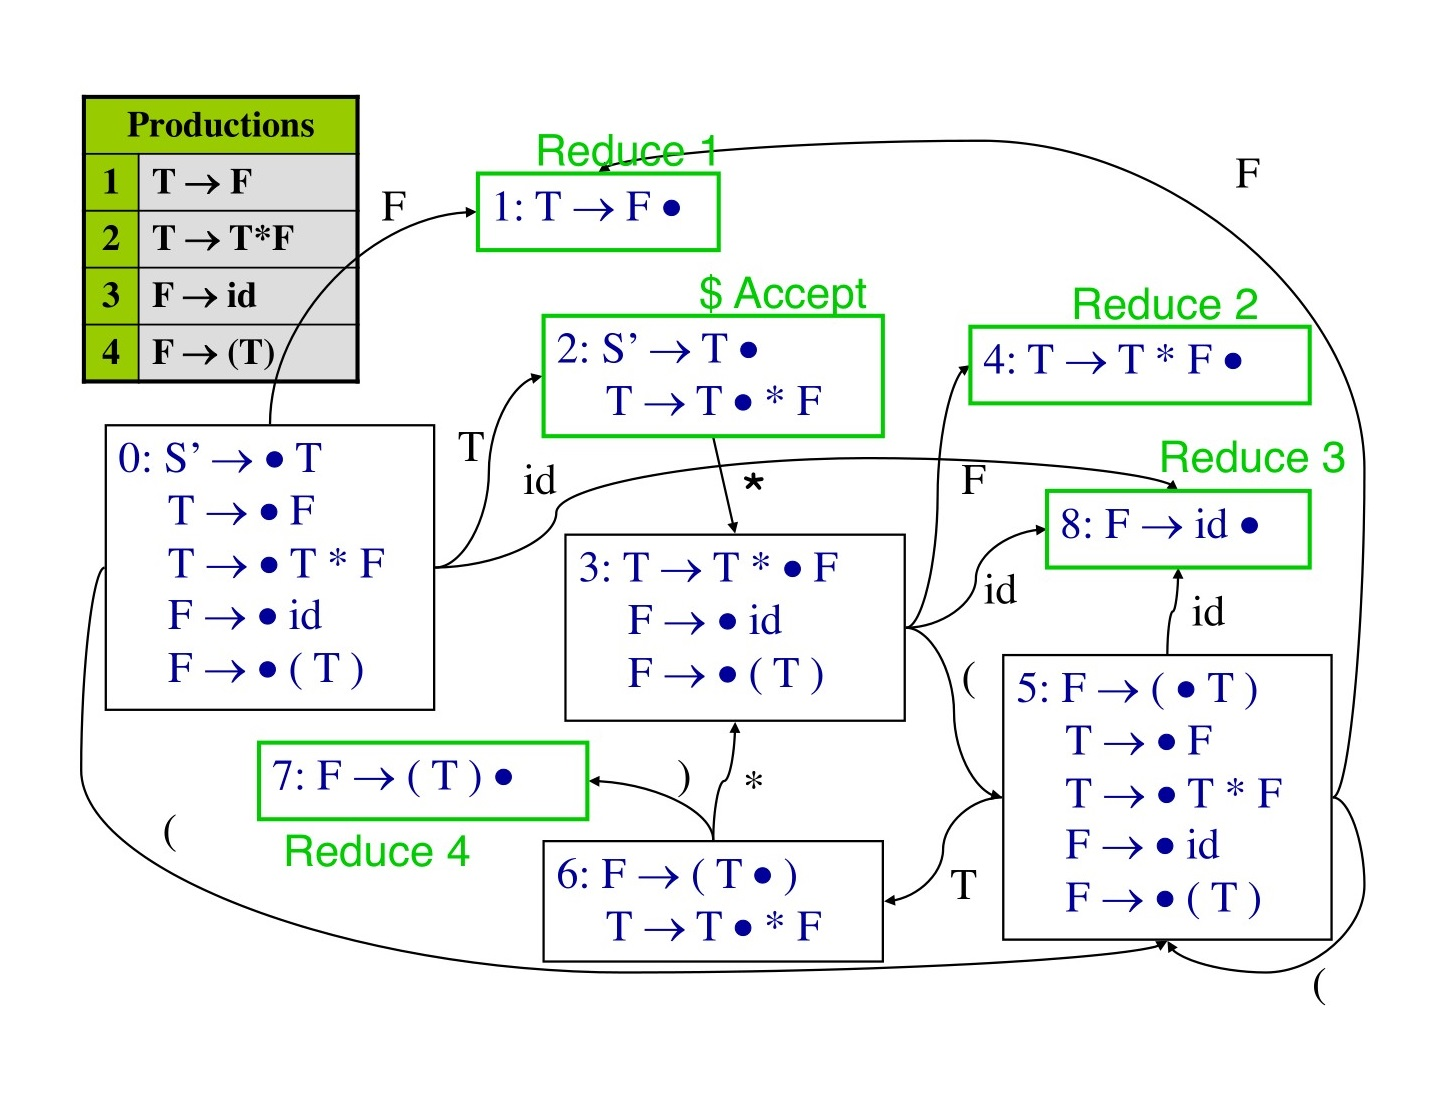
\includegraphics[width=\textwidth]{lrk-states-diagram}
	\end{center}
\end{figure}

	&& For an example diagram of a set of production rules (including epsilon rules) and the states generated using the successor function, see figure~\ref{fig:example-diagram-of-states-epsilon}

\begin{figure}[!htb]
	\caption{Example Diagram of States with Epsilon Rules}
	\label{fig:example-diagram-of-states-epsilon}
	\begin{center}
		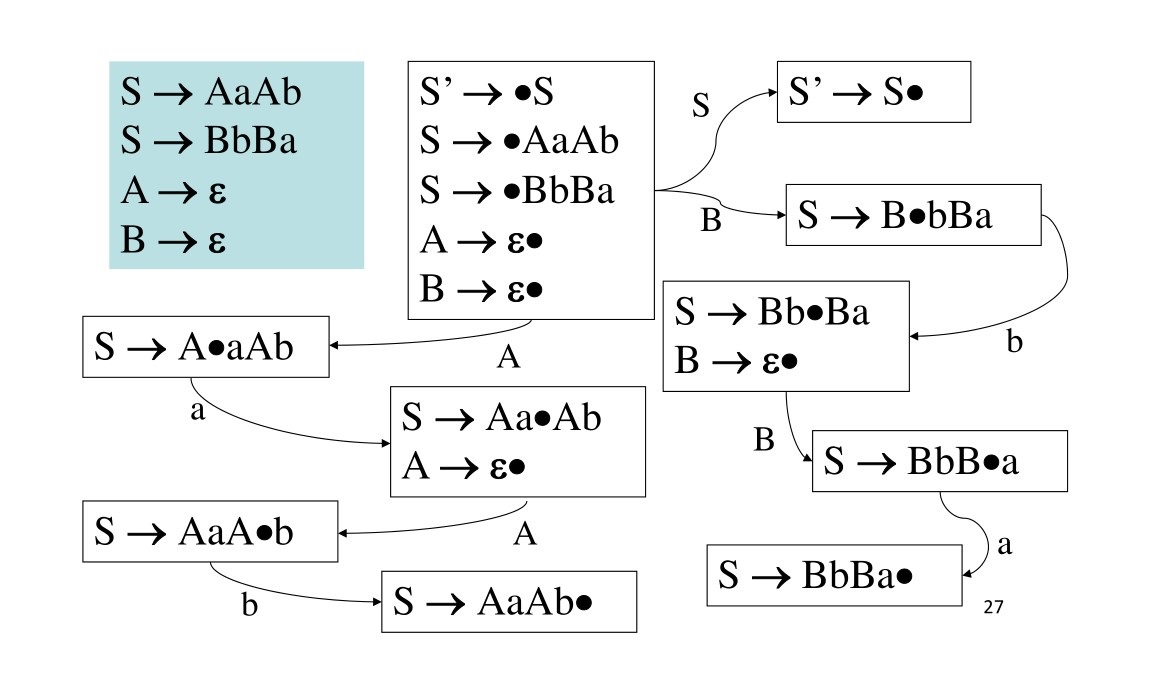
\includegraphics[width=\textwidth]{lrk-states-epsilon-diagram}
	\end{center}
\end{figure}

& \textbf{Viable prefix:} Set of states representing the stack of a shift-reduce parser where combining it with the remaining symbols is a valid state
	&& Notation: $\gamma$ such that $\gamma | \omega$ is a valid state for some $\omega$

& Process of LR(k) parsing:
	&& Requires a set of production rules, an action/goto table, and an input string
	&& Begin with state $0$ on the stack.
	&& From the row number of the current state (given by the top of the stack) and the leftmost symbol in the input, continually take the given action in the action table, given by $\textrm{action}[]$.
		&&& If the action is $S\alpha$, then push state $\alpha$ onto the stack and consume the leftmost symbol of the input.
		&&& If the action is $Rr$, then:
			&&&& Find the production rule numbered $r$, with $r: X \rightarrow Y_1 \dotsc Y_k$.
			&&&& Pop $k$ states from the stack.
			&&&& Take the state $Z$ at the top of the stack and push state $\textrm{goto}[Z, X]$ onto the stack.
		&&& If the action is $\textrm{ACCEPT}$, then complete the parsing.
		&&& If no action exists, then return $\textrm{ERROR}$.

	&& Example: Given the production rules in figure~\ref{tab:lrk-productions} and action/goto table in figure~\ref{tab:lrk-ag-table}, the trace of the LR(0) parse is figure~\ref{tab:lrk-trace}

\end{easylist}
\begin{figure}[!htb]
	\caption{LR(k) Parsing Example: Production Rules}
	\label{tab:lrk-productions}
	\begin{center}
		\begin{tabular}{ r | l }
			& Production Rules \\
			\hline
			1 & $T \rightarrow F$ \\
			2 & $T \rightarrow T*F$ \\
			3 & $F \rightarrow id$ \\
			4 & $F \rightarrow (T)$
		\end{tabular}
	\end{center}
\end{figure}
\begin{easylist}

\end{easylist}
\begin{figure}[!htb]
	\caption{LR(k) Parsing Example: Action/Goto Table}
	\label{tab:lrk-ag-table}
	\begin{center}
		\begin{tabular}{ r | c | c | c | c | c || c | c }
			\multirow{2}{*}{\textbf{States}} & \multicolumn{5}{ c || }{\textbf{Actions}} & \multicolumn{2}{c}{\textbf{Gotos}} \\
			& * & ( & ) & id & \$ & T & F \\
			\hline
			0 & & S5 & & S8 & 2 & 1 \\
			1 & R1 & R1 & R1 & R1 & R1 & \\
			2 & S3 & & & & ACC & \\
			3 & & S5 & & S8 & & 4 \\
			4 & R2 & R2 & R2 & R2 & R2 & \\
			5 & & S5 & & S8 & & 6 & 1 \\
			6 & S3 & & S7 & & & \\
			7 & R4 & R4 & R4 & R4 & R4 & \\
			8 & R3 & R3 & R3 & R3 & R3 &
		\end{tabular}
	\end{center}
\end{figure}
\begin{easylist}

\end{easylist}
\begin{figure}[!htb]
	\caption{LR(k) Parsing Example: Trace}
	\label{tab:lrk-trace}
	\begin{center}
		\begin{tabular}{ l | r | l }
			Stack & Input & Action \\
			\hline
			0 & (id)*id & Shift 5 \\
			0, 5 & id)*id & Shift 8 \\
			0, 5, 8 & )*id & Reduce using production rule 3: $F \rightarrow id$ \\
			&& Pop 1 symbol from the stack (8) \\
			&& Push $goto[5, F] = 1$ onto the stack \\
			0, 5, 1 & )*id & R1: $T \rightarrow F$ \\
			&& Pop 1 \\
			&& $goto[5, T] = 6$ \\
			0, 5, 6 & )*id & S7 \\
			0, 5, 6, 7 & *id & R4, $F \rightarrow (T)$ \\
			&& Pop 7, 6, 5 \\
			&& $goto[0, T] = 1$ \\
			0, 1 & *id & R1: $T \rightarrow F$ \\
			&& Pop 1 \\
			&& $goto[0, T] = 2$ \\
			0, 2 & *id & S3 \\
			0, 2, 3 & id & S8 \\
			0, 2, 3, 8 & \$ & R3: $F \rightarrow id$ \\
			&& Pop 8 \\
			&& $goto]3, F] = 4$ \\
			0, 2, 3, 4 & \$ & R2: $T \rightarrow T*F$ \\
			&& Pop 4, 3, 2 \\
			&& $goto[0, T] = 2$ \\
			0, 2 & \$ & ACCEPT
		\end{tabular}
	\end{center}
\end{figure}
\begin{easylist}

\end{easylist}
\subsection{LR(0) Parsing}
	\label{subsec:parsing-algorithms-bottom-up:lr0}
\begin{easylist}

& \textbf{LR(0) parsing:} Form of LR(k) parsing where no tokens of lookahead are used, so a reduction is always executed whenever possible
	&& \textbf{LR(0) grammar:} Subset of CFGs where an LR(0) construction can be generated without shift-reduce or reduce-reduce conflicts (i.e. the generated pushdown automata is deterministic)

& Grammar validity:
	&& A grammar is LR(0) if and only if no shift-reduce or reduce-reduce conflicts exist in the itemsets
	&& A grammar is not LR(0) if and only if at least one shift-reduce or reduce-reduce conflict exists in the itemsets

\end{easylist}
\subsection{SLR(1) Parsing}
	\label{subsec:parsing-algorithms-bottom-up:slr1}
\begin{easylist}

& \textbf{LR(1) parsing:} Form of LR(k) parsing where 1 token of lookahead is available for use

& \textbf{SLR(1)/SLR/Simple LR parsing:} Subset of LR(0) parsing where each \textit{production rule} includes all possible $FOLLOW$ terminal symbols using 1 character of lookahead

& \textbf{SLR(1)/SLR/Simple LR grammar:} Subset of CFGs where an LR(1) construction can be generated without shift-reduce or reduce-reduce conflicts, or conflicts exist but can be resolved due to having a single $FOLLOW$ symbol
	&& First/follow:
		&&& \textbf{First:} Set of terminal symbols which are the beginning symbols of all strings which can be derived from a given symbol
			&&&& Notation: $FIRST(S) = \{a, b\}$ where $S$ is a given symbol and $a, b$ are terminal symbols
			&&&& Example: Given a set of production rules, the First sets of the non-terminal symbols are derived in table~\ref{tab:first-example}
		&&& \textbf{Follow:} Set of terminal symbols which can follow a given symbol
			&&&& Notation: $FOLLOW(S) = \{a, b\}$ where $S$ is a given symbol and $a, b$ are terminal symbols
			&&&& Example: Given a set of production rules, the Follow sets of the non-terminal symbols are derived in table~\ref{tab:follow-example}
		&&& Example: Given a set of production rules, the First and Follow sets of the non-terminal symbols can be derived as follows:
			&&&& See table~\ref{tab:first-follow-sets-example-1}
			&&&& See table~\ref{tab:first-follow-sets-example-2}

\end{easylist}
\begin{figure}[!htb]
	\caption{First Example}
	\label{tab:first-example}
	\begin{center}
		\begin{tabular}{ r l }
			Production Rules:
			& $A \rightarrow Bc | d$ \\
			& $B \rightarrow e$ \\
			\hline
			$FIRST(A) =$ & $\{d, e\}$ \\
			$FIRST(B) =$ & $\{e\}$
		\end{tabular}
	\end{center}
\end{figure}
\begin{easylist}

\end{easylist}
\begin{figure}[!htb]
	\caption{Follow Example}
	\label{tab:follow-example}
	\begin{center}
		\begin{tabular}{ r l }
			Production Rules:
			& $A \rightarrow Bc$ \\
			& $B \rightarrow Bd | BC$ \\
			& $C \rightarrow e$ \\
			\hline
			$FOLLOW(A) =$ & $\{ \$ \}$ \\
			$FOLLOW(B) =$ & $\{c, d, e\}$ \\
			$FOLLOW(C) =$ & $\{c\}$
		\end{tabular}
	\end{center}
\end{figure}
\begin{easylist}

\end{easylist}
\begin{figure}[!htb]
	\caption{First/Follow Sets Example 1}
	\label{tab:first-follow-sets-example-1}
	\begin{center}
		\begin{tabular}{ r | l }
			Production Rules
			& $S \rightarrow AB$ \\
			& $A \rightarrow c | \epsilon$ \\
			& $B \rightarrow cbB | a$ \\
			\hline
			First sets
			& $FIRST(A) = \{c, \epsilon\}$ \\
			& $FIRST(B) = \{c, a\}$ \\
			& $FIRST(S) = FIRST(A) = \{c, \epsilon\}$ \\
			\hline
			Follow sets
			& $FOLLOW(A) = FIRST(B) = \{c, a\}$ \\
			& $FOLLOW(B) = \{\$\}$ \\
			& $FOLLOW(S) = \{\$\}$
		\end{tabular}
	\end{center}
\end{figure}
\begin{easylist}

\end{easylist}
\begin{figure}[!htb]
	\caption{First/Follow Sets Example 2}
	\label{tab:first-follow-sets-example-2}
	\begin{center}
		\begin{tabular}{ r | l }
			Production Rules
			& $S \rightarrow cAa$ \\
			& $A \rightarrow cB | B$ \\
			& $B \rightarrow bcB | \epsilon$ \\
			\hline
			First sets
			& $FIRST(A) = \{c, b, \epsilon\}$ \\
			& $FIRST(B) = \{b, \epsilon\}$ \\
			& $FIRST(S) = \{c\}$ \\
			\hline
			Follow sets
			& $FOLLOW(A) = \{a\}$ \\
			& $FOLLOW(B) = FOLLOW(A) = \{a\}$ \\
			& $FOLLOW(S) = \{\$\}$
		\end{tabular}
	\end{center}
\end{figure}
\begin{easylist}

	&& Process to determine whether a shift-reduce conflict can be eliminated by a 1-token lookahead:
		&&& Find the $FOLLOW$ set of the reduce rule
		&&& Find the next accepted symbol of the shift rule
		&&& If the symbol is in the $FOLLOW$ set, then the conflict cannot be eliminated
		&&& Example: Given the set of production rules in table~\ref{tab:slr-shift-reduce}, the state $S \rightarrow A \bullet xB; B \rightarrow A \bullet$ has a shift-reduce conflict which cannot be resolved by 1 token of lookahead, as the parser can still shift or reduce on $x$ because the $FOLLOW$ set of $B$ is $\{ x, \$ \}$

\end{easylist}
\begin{figure}[!htb]
	\caption{SLR Shift-Reduce Conflict Example}
	\label{tab:slr-shift-reduce}
	\begin{center}
		\begin{tabular}{ l }
			$S \rightarrow Ax$ \\
			$S \rightarrow B$ \\
			$B \rightarrow A$ \\
			$A \rightarrow yB$
		\end{tabular}
	\end{center}
\end{figure}
\begin{easylist}

	&& Example: Given the set of production rules and transition diagram in figure~\ref{fig:slr-1-parsing-prod-rules-diagram}, the trace of the SLR(1) parse of $id * id$ is table~\ref{tab:slr-1-parsing-trace}

\begin{figure}[!htb]
	\caption{SLR(1) Parsing Example: Production Rules and Diagram}
	\label{fig:slr-1-parsing-prod-rules-diagram}
	\begin{center}
		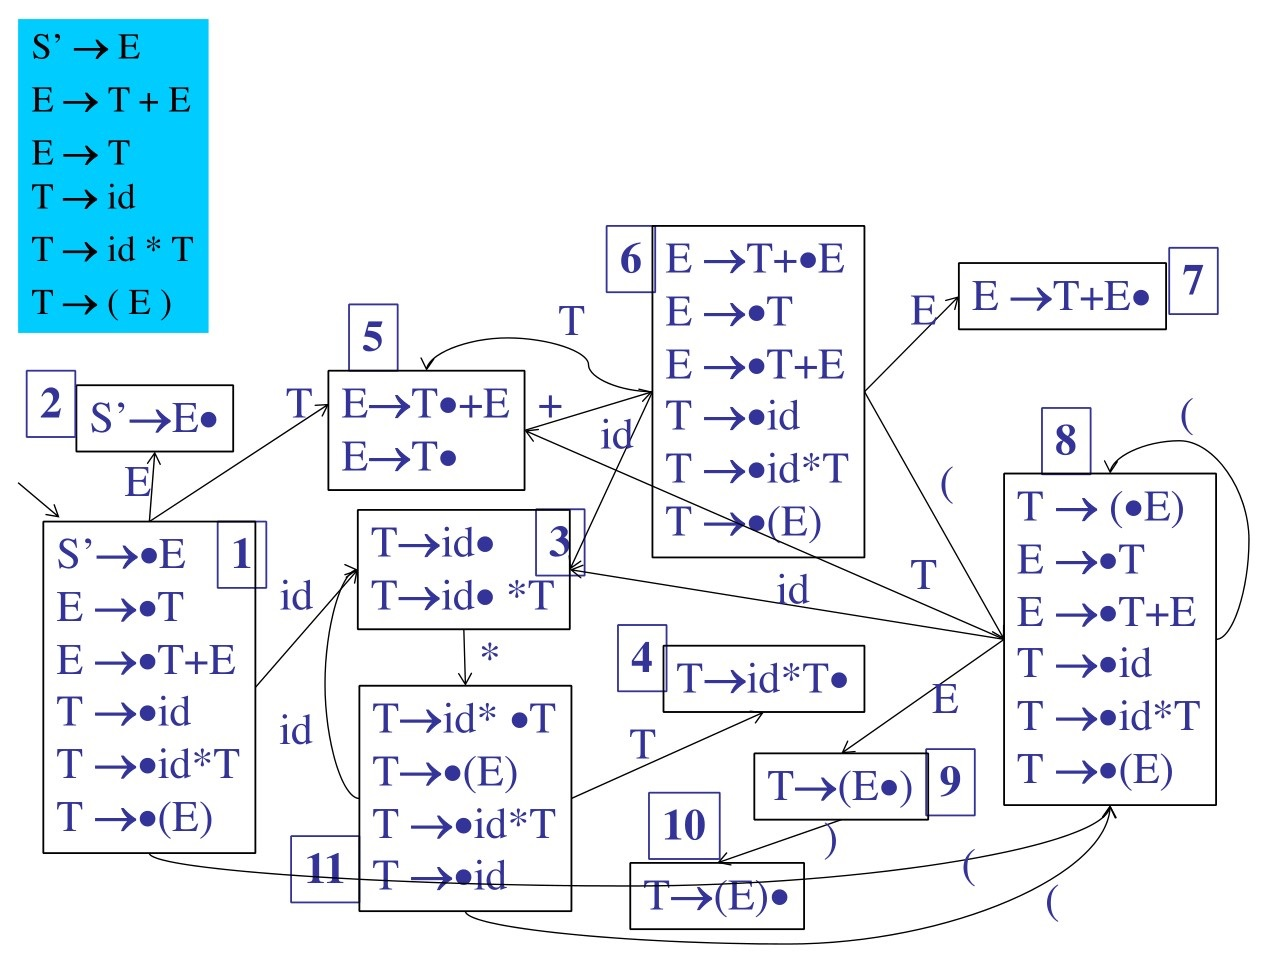
\includegraphics[width=\textwidth]{slr-1-trace-diagram}
	\end{center}
\end{figure}

\end{easylist}
\begin{figure}[!htb]
	\caption{SLR(1) Parsing Example: Trace}
	\label{tab:slr-1-parsing-trace}
	\begin{center}
		\begin{tabular}{ l | r | l }
			Stack and Input & DFA Halt State & Action \\
			\hline
			$| id * id\$ $ & $1$ & Shift \\
			$id | * id\$ $ & $3 ( \* \not\in FOLLOW(T) )$ & Shift \\
			$id * | id\$ $ & $11$ & Shift \\
			$id * id |\$ $ & $3 (\$ \in FOLLOW(T) )$ & Reduce $T \rightarrow id$ \\
			$id * T | \$ $ & $4 (\$ \in FOLLOW(T) )$ & Reduce $T \rightarrow id * T$ \\
			$T | \$ $ & $5 (\$ \in FOLLOW(T) )$ & Reduce $E \rightarrow T$ \\
			$E | \$ $ & & Accept
		\end{tabular}
	\end{center}
\end{figure}
\begin{easylist}

& Grammar validity:
	&& A grammar is SLR(1) if and only if, for each shift-reduce or reduce-reduce conflict in the configuration sets, the $FOLLOW$ sets of the conflicting production rules (not dotted rules) do not intersect
	&& A grammar is not SLR(1) if and only if there exists at least one shift-reduce or reduce-reduce conflict in the configuration sets where the $FOLLOW$ sets of the conflicting production rules intersect

\end{easylist}
\subsection{Canonical LR(1) Parsing}
	\label{subsec:parsing-algorithms-bottom-up:canonical-lr1}
\begin{easylist}

& \textbf{LR(1)/Canonical LR(1) parsing:} Subset of LR(0) parsing where each \textit{dotted rule} includes a 1-character lookahead, rather than each production rule
	&& More accurate than SLR(1) parsing
	&& Notation: $\textrm{dotted rule, } \alpha / \beta$ where $\alpha, \beta$ are the potential $FOLLOW$ characters of the non-terminal symbol if the rule was parsed and reduced
	
& Grammar validity:
	&& A grammar is LR(1) if and only if, for each shift-reduce or reduce-reduce conflict, the $FOLLOW$ sets of the dotted rules do not conflict
	&& A grammar is not LR(1) if and only if there exists at least one itemset where conflicting dotted rules have intersecting $FOLLOW$ sets

\end{easylist}
\subsection{LALR(1) Parsing}
	\label{subsec:parsing-algorithms-bottom-up:lalr1}
\begin{easylist}

& \textbf{LALR(1) parsing:} Subset of LR(0) parsing which combines states when they share the same dotted rules but have different $FOLLOW$ sets
	&& More specific than SLR(1) (as resulting $FOLLOW$ sets may not always be the complete \\ $FOLLOW$ set)
	&& Simplified/compact version of canonical LR(1)
	
& Grammar validity:
	&& A grammar is LALR(1) if and only if, when states with matching dotted rules are merged, for each combination of states, for each matching dotted rule in the resulting configuration set, there are no conflicts in the 1-character lookaheads
	&& A grammar is not LALR(1) if and only if, when states with matching dotted rules are merged, the $FOLLOW$ sets contain shift-reduce or reduce-reduce conflicts

\end{easylist}
\clearpage

	%
% CMPT 379: Principles of Compiler Design - A Course Overview
% Section: Parsing Algorithms: Top-Down
%
% Author: Jeffrey Leung
%

\section{Parsing Algorithms: Top-Down}
	\label{sec:parsing-algorithms-top-down}
\subsection{Introduction}
	\label{subsec:parsing-algorithms-top-down:introduction}
\begin{easylist}

& \textbf{Top-down/leftmost parsing:} Deterministic creation of a string beginning from a start symbol and continuously expanding the leftmost non-terminal symbol
	&& Similarly efficient to bottom-up parsing
	&& Constructs a parse tree by expanding symbols from the top to the bottom, left to right
	&& As shifts and reduces are not valid actions, neither shift-reduce nor reduce-reduce conflicts are possible

\end{easylist}
\subsection{Recursive Descent Parsing}
	\label{subsec:parsing-algorithms-top-down:recursive-descent-parsing}
\begin{easylist}

& \textbf{Recursive descent parser:} Top-down parser which applies any valid production rule to the leftmost non-terminal symbol and, when no option are valid, backtracks in a brute-force manner until a valid construction is parsed (i.e. backtracking search)
	&& Efficient when using a grammar which is:
		&&& Unambiguous
		&&& Left-factored
		&&& Free of left-recursion

& \textbf{Left-recursive grammar:} Grammar which recurses using a symbol on the left of the production rule string
	&& E.g. $A \rightarrow Ab | c$ is left-recursive
	&& Causes top-down parsers to create infinite loops
	&& E.g. Given left-recursive grammar $A \rightarrow A * B | B; B \rightarrow a$, an equivalent non-left-recursive grammar would be $X \rightarrow BA; A \rightarrow *BA | \epsilon; B \rightarrow a$
	&& E.g. Given a set of production rules, figure~\ref{tab:left-recursion-example} shows the steps to remove left-recursion

\end{easylist}
\begin{figure}[!htb]
	\caption{Elimination of Left-Recursion: Example}
	\label{tab:left-recursion-example}
	\begin{center}
		\begin{tabular}{ r | l }
			Production Rules
			& $S \rightarrow Aa|b$ \\
			& $A \rightarrow Ac | Sd | \epsilon$ \\
			\hline
			Remove $A \rightarrow S$ recursion
			& $S \rightarrow Aa|b$ \\
			& $A \rightarrow bd A' | A'$ \\
			& $A' \rightarrow A'c | A' ad$ \\
			\hline
			Remove $A'$ left-recursion
			& $S \rightarrow Aa|b$ \\
			& $A \rightarrow bd A' | A'$ \\
			& $A' \rightarrow cA' | adA'$
		\end{tabular}
	\end{center}
\end{figure}
\begin{easylist}

& \textbf{Left-factoring:} Operation on a grammar which combines all common strings on the leftmost of a production rule string
	&& Left-factored grammars create ambiguous rule expansions as a given terminal can expand to multiple potential states
	&& E.g. Given grammar $A \rightarrow Bc | D; B \rightarrow ef; D \rightarrow e$, left-factoring would create the grammar $A \rightarrow eB; B \rightarrow fc | \epsilon$

\end{easylist}
\subsection{LL(1) Parsing}
	\label{subsec:parsing-algorithms-top-down:ll1-parsing}
\begin{easylist}

& \textbf{LL(1) parsing:} Top-down parsing algorithm which creates a left-to-right leftmost derivation requiring only 1 symbol of lookahead
	&& Requires a grammar which is:
		&&& Unambiguous
		&&& Left-factored
		&&& Free of left-recursion
	&& Only one possible production can exist given the next token

& \textbf{Predictive parsing table:} Table which correlates the leftmost non-terminal symbol and the next terminal symbol with the only possible production
	&& No cell can have more than one string as the expansion to the rule
	&& Empty cells mean parsing errors
	&& Uses lookahead to resolve conflicts between multiple possible production rule applications for the same symbol
	&& Layout: See figure~\ref{tab:predictive-parsing-table-layout}

\end{easylist}
\begin{figure}[!htb]
	\caption{Predictive Parsing Table Layout}
	\label{tab:predictive-parsing-table-layout}
	\begin{center}
		\begin{tabular}{ r r | l l }
			& & \textbf{Terminal symbols} & \$ \\
			\hline
			\textbf{Non-terminal Symbols} & \textit{Symbol} & \textit{Production result}
		\end{tabular}
	\end{center}
\end{figure}
\begin{easylist}

& To create a predictive parsing table:
	&& For each non-terminal symbol $X$ on the left column:
		&&& If there is a production rule where $X$ expands to epsilon ($\epsilon$), then:
			&&&& For each terminal symbol which is in the $FOLLOW$ of symbol $X$, write $\epsilon$
		&&& If there is a production rule where $X$ expands to a string which is not epsilon ($\epsilon$), then:
			&&&& For each terminal symbol which is in the $FIRST$ of symbol $X$, write the expansion of the valid production rule

& E.g. In figure~\ref{tab:ll1-conflict-resolution}, $Y \rightarrow \epsilon$ is the valid production rule to be chosen when $+, ),$ or $\$$ are the lookahead symbol

\end{easylist}
\begin{figure}[!htb]
	\caption{LL(1) Conflict Resolution with $FOLLOW$}
	\label{tab:ll1-conflict-resolution}
	\begin{center}
		\begin{tabular}{ r l }
			Production Rules
			& $E \rightarrow TX$ \\
			& $X \rightarrow \epsilon$ \\
			& $X \rightarrow +E$ \\
			& $T \rightarrow (E)$ \\
			& $T \rightarrow id Y$ \\
			& $Y \rightarrow *T$ \\
			& $Y \rightarrow \epsilon $ \\
			\hline
			$FOLLOW(Y)$
			& $= FOLLOW(T)$ \\
			& $= ( FIRST(X) - \{\epsilon\} ) + FOLLOW(E)$ \\
			& $= \{ +, ), \$ \}$
		\end{tabular}
	\end{center}
\end{figure}
\begin{easylist}
	
& LL(1) parsing trace:
	&& Stack is used to keep track of non-terminal symbols
	&& Stack and input strings are terminated with the end of input symbol (\$)
	&& Layout: See figure~\ref{tab:ll1-parsing-trace-example}

\end{easylist}
\begin{figure}[!htb]
	\caption{LL(1) Parsing Trace Example}
	\label{tab:ll1-parsing-trace-example}
	\begin{center}
		\begin{tabular}{ l | l | l }
			\textbf{Stack} & \textbf{Input} & \textbf{Action} \\
			\hline
			\textit{string \$} & \textit{string \$} & \textit{Production rule to expand OR} \\
			&& \textit{$\epsilon$ OR} \\
			&& \textit{Terminal $\alpha$ OR} \\
			&& \textit{acc}
		\end{tabular}
	\end{center}
\end{figure}
\begin{easylist}

	&& To create an LL(1) parsing trace:
		&&& For the leftmost input symbol and the leftmost stack symbol:
			&&&& If the leftmost stack symbol is a non-terminal symbol, then use the leftmost input and stack symbols to find the corresponding production rule expansion from the predictive parsing table, and:
				&&&&& If the expansion is not an epsilon, then replace the leftmost stack symbol with the expansion
				&&&&& If the expansion is an epsilon ($\epsilon$), then remove the leftmost stack symbol
			&&&& If the leftmost stack symbol is a terminal symbol and the leftmost stack and input symbols match, then consume both of them with the action \textit{Terminal}
			&&&& If the leftmost stack and input symbols are the end of input (\$), then accept the parse

& Grammar validity:
	&& A grammar is LL(1) if and only if, for each pairing of a non-terminal symbol with a terminal symbol, only one possible production rule can be applied
	&& A grammar is not LL(1) if and only if there exists at least one pairing of a non-terminal symbol and a terminal symbol which can expand to multiple production rules (e.g. $A \rightarrow bc; A \rightarrow bd$)

\end{easylist}
\clearpage

	%
% CMPT 379: Principles of Compiler Design - A Course Overview
% Section: Syntax-Directed Transmission
%
% Author: Jeffrey Leung
%

\section{Syntax-Directed Transmission}
	\label{sec:syntax-directed-translation}
\begin{easylist}

& \textbf{Syntax-Directed Transmission:} Compiler implementation where the parser conveys and passes information between syntax trees
	&& Generalization of a CFG where each symbol includes an additional attribute

& \textbf{Attribute grammar:} Set of syntax-directed rules which construct a meaning from a set of strings
	&& Addition to a parse tree
	&& \textbf{Decorate/annotate:} Description of the effect of an attribute grammar on a parse tree

& \textbf{Attribute:} Arbitrary value assigned to each symbol representation
	&& \textbf{Synthesized attribute:} Parse tree attribute which is determined by the attribute value(s) of the child nodes
	&& \textbf{Inherited attribute:} Parse tree attribute which is determined by the attribute value(s) of the parent and/or sibling nodes
		&&& E.g. Parent action \lstinline|{ $$.in = 3; }|, child action \lstinline|{ print($0.in); }|

& \textbf{S-attributed definition:} Semantic-action grammar with only synthesized attributes
& \textbf{L-attributed definition:} Semantic-action grammar where, for each production \\ $A \rightarrow B_1 \ldots B_{j-1} B_{j} \ldots B_{n}$, for each $j = 1 \ldots n$, each inherited attribute of $B_j$ depends on the inherited attributes of $A$ and the attributes of $B_1 \ldots B_{j-1}$
	&& Superset of S-attributed definitions

\end{easylist}
\clearpage

	%
% CMPT 379: Principles of Compiler Design - A Course Overview
% Section: Semantic Analysis and Static Single Assignment
%
% Author: Jeffrey Leung
%

\section{Semantic Analysis and Static Single Assignment}
	\label{sec:semantic-analysis-ssa}
\begin{easylist}

& \textbf{Semantic analysis:} Validating a program's basic requirements and type compatibilities, processing static semantic checks, and adding run-time semantic checks
	&& E.g. Checking that a \textit{main} function exists, that variables are declared, whether operand types are compatible

& \textbf{Static Single Assignment (SSA):} Property of an intermediate representation where each variable is only assigned once
	&& Used to distinguish and merge values from multiple possible paths of computation to create a single resulting value

& \textbf{Dominance:} Characteristic of a node which is a mandatory predecessor of another node (i.e. any path from the root to the lower node must pass through the upper node)
	&& Any node dominates itself
	&& Definitions of a variable dominate its later usages
	&& \textbf{Strict dominance:} Characteristic of a node which dominates a different node

& \textbf{Dominance Frontier (DF):} Set of nodes which, given a target node, are the convergence of two nodes - one which is dominated by the target node and one which is not (i.e. all nodes such that the target node dominates a predecessor but not the node itself)
	&& Notation: $DF(X)$
	&& Can include the node itself
	&& E.g. See figure~\ref{fig:dominance-frontier-example} which calculates the dominance frontier of node 5

\begin{figure}[!htb]
	\caption{Dominance Frontier Example}
	\label{fig:dominance-frontier-example}
	\begin{center}
		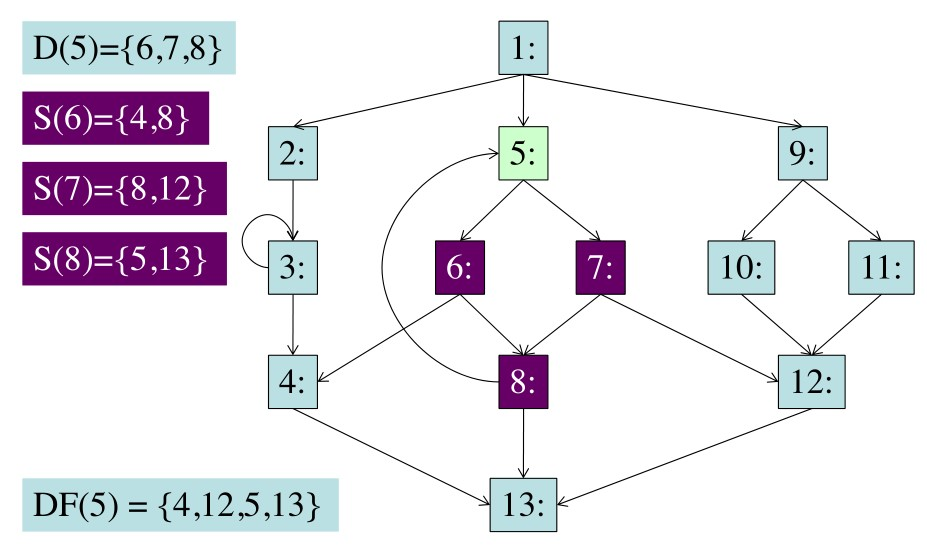
\includegraphics[width=\textwidth]{dominance-frontier}
	\end{center}
\end{figure}

	&& Every node in $DF(X)$ requires a $\phi$ (phi) function for each variable defined in $X$

& \textbf{Dominator tree:} Acyclical hierarchical structure of a set of nodes, where a node dominates all of its children

\end{easylist}
\clearpage

	%
% CMPT 379: Principles of Compiler Design - A Course Overview
% Section: Programming Language Structure
%
% Author: Jeffrey Leung
%

\section{Programming Language Structure}
	\label{sec:programming-language-structure}
\begin{easylist}

& \textbf{Procedure:} Series of computational steps to be executed
	&& Assumption that execution is sequential (which can be violated by concurrency)
	&& Assumption that control is returned to the caller after execution (which can be violated by exceptions)
	&& \textbf{Activation:} Invocation of a given procedure
		&&& \textbf{Activation tree:} Tree of invoked procedures where each child node was invoked by its parent node
	&& \textbf{Lifetime (procedure):} Set of all the steps required to execute the associated procedure and its subprocedures
	&& Stack is used to keep track of all procedures which are currently active

& \textbf{Control Flow Graph (CFG):} Diagram showing logic flow of code, with branching on conditional commands such as if/for/while loops

\end{easylist}
\clearpage

	%
% CMPT 379: Principles of Compiler Design - A Course Overview
% Section: Optimization
%
% Author: Jeffrey Leung
%

\section{Optimization}
	\label{sec:optimization}
\begin{easylist}

& \textbf{Constant folding:} Compile-time preprocessing of constant values to avoid predictable runtime computation
& \textbf{Constant propagation:} If a variable is set to a constant, then replace all future variable uses with the constant (until the variable is reassigned)
& \textbf{Copy propagation:} Simplification of multiple computations of the same values
& \textbf{Dead code elimination:} Removal of code which will never be executed, used, or have any side effects

& \textbf{Algebraic simplification:} Basic arithmetic and algebraic simplifications which are computed during compile-time such as addition by 0 or multiplication by 0 or 1
& \textbf{Reduction of strength:} Replacement of exponentiation with multiplication

& Correctness: Optimizations must not change the meaning of a performance

\end{easylist}
\clearpage

	%
% CMPT 379: Principles of Compiler Design - A Course Overview
% Section: Register Allocation
%
% Author: Jeffrey Leung
%

\section{Register Allocation}
	\label{sec:register-allocation}
\begin{easylist}

& Intermediate representation uses unlimited temporary storage locations, which must be translated to a limited number of registers
& \textbf{Live:} Variable which has been defined and is being used or will be used later
	&& Should be loaded into a register for quicker access
& \textbf{Liveness analysis:} Detection of when variables are and are not live
	&& Variables can share a register if, at all points in the program, no more than one of them are live
	&& At the end of each line of code, create a set of all live variables
	&& \textbf{Live range:} Locations in the program where a variable is live
	&& \textbf{Live interval:} Start and end line numbers which represent from when a variable is first defined to its last usage
		&&& Greedy algorithm can be applied to allocate registers based on when the live interval for a variable ends

& \textbf{Register Interference Graph (RIG):} Undirected graph where each node represents a unique temporary variable, and an edge $(t_1, t_2)$ exists iff they are both live at any given point in the program
	&& For two variables $v_1, v_2$, if there is no edge connecting them, they can be allocated to the same register
	&& E.g. For the RIG in figure~\ref{fig:example-register-interference-graph}, $a, c$ cannot be in the same register, but $a, d$ can be in the same register

\begin{figure}[!htb]
	\caption{Example of a Register Interference Graph}
	\label{fig:example-register-interference-graph}
	\begin{center}
		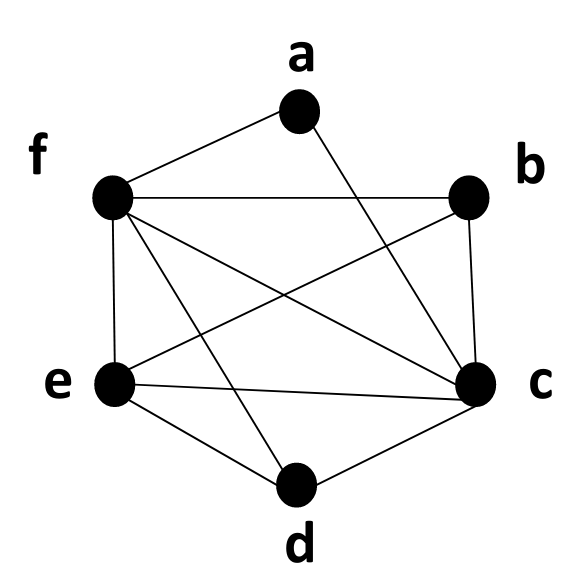
\includegraphics[width=0.4\textwidth]{register-interference-graph.png}
	\end{center}
\end{figure}

& \textbf{Spilling:} Operation which allocates a memory location for a variable when there are not enough registers to store all live variables
	&& When a variable must be spilled, the live range of the variable is reduced and the RIG is updated

& $k$-coloring problem: Given a graph, can $k$ colors be applied to the nodes such that each node has only one color, and no connected nodes share the same color?
	&& Apply the $k$-coloring problem to find the minimum possible coloring for the graph, where $k$ also equals the minimum number of registers required
	&& If $k$ is not large enough, then a node is spilled
	&& \textit{Optimistic coloring heuristic algorithm:}
		&&& Choose an arbitrary $k$ to attempt
		&&& Remove a node with less than $k$ neighbors and push it into a stack (repeat until the graph is empty)
		&&& Pop a node and connect it to its neighbors in the graph, then assign either an existing color or a new color (repeat until the stack is empty)

& \textbf{Linear scan register alllocation:} Algorithm which detects when a variable needs to be spilled
	&& Efficient
	&& Less effective than graph coloring

\end{easylist}
\clearpage


\end{document}
